% !TeX root = ../main.tex
% Add the above to each chapter to make compiling the PDF easier in some editors.

\chapter{Evaluation}\label{chapter:evaluation}

This section provides an evaluation of the designed artifact in two ways. In the previous section, seven requirements have been defined for the designed system. First, it will be discussed how the designed system fits in these requirements. Second, a qualitative evaluation of the system will be presented. For this part of the evaluation, one hour interviews with five different researchers with peer review experience were conducted. The \acrfull{TAM} is used as a framework to assess the system usage qualitatively. The responses by the interviewees are categorized under \acrshort{TAM} variables and interpreted to determine their intention to use of the system. According to the responses, a basic \acrlong{TAM} is proposed. Various insights gained during the interviews about the system and peer reviewing in general are also shared.

\section{Evaluation of Design Requirements}

Based on open science principles and the problems discussed, seven requirements were defined for the system:

\begin{itemize}
  \item RQ1: Verifiability 
  \item RQ2: Transparency 
  \item RQ3: Open Data 
  \item RQ4: Open Standards 
  \item RQ5: Direct Trust 
  \item RQ6: Selective Disclosure 
  \item RQ7: Compatibility 
\end{itemize}

\subsubsection{1. Verifiability}

Verifiability, in short, encompasses the ability to check if a peer review has really taken place and the presented information about the peer review is correct. The designed system is based on \acrlong{VC}, which makes use of the Linked-Data Proofs or \acrshort{JSON} Web Tokens that allows the verification of credentials using digital signatures. By resolving the \lstinline{issuer} (journal) identifier, their public keys can be retrieved and the credential can be verified. 

\subsubsection{2. Transparency}

The designed system improves upon the existing ones in numerous ways in terms of transparency. First of all, the verification of the peer reviews is transparent, that is anyone can take the existing data and verify that the peer review credential is actually issued by the given journal, and that it is authentic. Current showcasing platforms verify the reviews themselves and mark the reviews as verified without information on how this verification is done. Also, the Veriview platform can complete the verification steps and inform the users on its user interface that the review is verified. By open sourcing the code this process is also kept transparent.

\subsubsection{3. Open Data}

Even though the nature of blinded peer reviews prevents complete openness of the data, the system makes it possible to keep as much data of peer reviews as possible open without losing verifiability. Additionally, the data stored in Veriview is identical to what is publicly available. 

\subsubsection{4. Open Standards}

The system is based on open standards under development such as \acrlong{VC}, \acrlong{DID}, \acrshort{JSON-LD}. The platforms are open sourced and anyone can easily create a similar platform. This would avoid future vendor lock-in and further contributes the openness of the system.

\subsubsection{5. Direct Trust}

The peer review credentials are issued directly by journals and the verification is also done through journal keys. The showcasing system only serves as a platform to share and host the credentials, and requires minimal trust. 

\subsubsection{6. Selective Disclosure}

By using Linked-Data Proofs with BBS+ Signatures, it is possible to derive credentials with a subset of the attributes, and with a zero-knowledge proof that ensures the knowledge of the original credential and a valid signature. This enables review authors to only share the non-identifiable information of a review without losing verifiability.

\subsubsection{7. Compatibility}

The proposed system allows the extension of the proposed peer review vocabulary or the use of different vocabularies instead. This enables to accommodate the data model of the credentials to different peer review processes but also keeps the interoperability by having the vocabularies published. 

\section{Interviews}

\subsection{Method}

For the qualitative evaluation of the work, five different researchers with peer review experience were interviewed. All participants were male. Four participants were invited for interviews through existing connections. Additionally, to at least interview one frequent Publons user, the researchers with most reviews under the "Researchers" tab on Publons were browsed. Among them 20 researchers were contacted who have at least one publication with an arbitrary order. In the end Interviewee 5 accepted the request to interview. Additional details on interviewee profiles are given in Table \ref{tab:interviewees}. Here the number of publications are taken from their Google Scholar profiles, and their peer review numbers from their statements if a Publons profile is not available. The interviews took around one hour, were recorded and transcribed with the interviewees' consents. The interviews encompassed first a general discussion around the interviewee's peer review experience and their perspectives, followed by an introduction to existing review showcasing platforms, in particular Publons, and their experience if they had any. Next, the conceptual design of the system is presented. The interviewees were then given a hands-on experience of the prototype and they were asked to complete the basic user flow of the application. Finally, their review of the system is solicited. 

\begin{table}[]
    \centering
    \begin{tabular}{c|c|c|c|c|c}
         & Field & Gender & Publications & Peer Reviews & Publons user? \\
         \hline
         Interviewee 1 & Computer Science & Male & 9 & 5-10 & Yes \\
         Interviewee 2 & Political Science & Male & 12 & 19 & No \\
         Interviewee 3 & Computer Science & Male & 13 & not stated & No \\
         Interviewee 4 & Theoretical Biology & Male & 52 & 40+ & No \\
         Interviewee 5 & Additive Manufacturing & Male & 97 & 816 & Yes \\
    \end{tabular}
    \caption{Interviewee details}
    \label{tab:interviewees}
\end{table}

The interviews were run as free dialogues and did not follow a strict structure besides the flow described above. However, the following or similar questions were asked to interviewees over the course of the interviews:

\begin{itemize}
    \item Could you please introduce yourself and detail your peer review experience?
    \item How would you describe the peer review culture in your field?
    \item What motivates you to do the peer review for a manuscript?
    \item Has there been a case where you presented your reviews in an academic resume, or that it would be beneficial if you could present it?
    \item Are you using review showcasing platforms? If yes, could you describe your experiences?
    \item What consequences may arise in the future that Publons is the only owner of the peer review data?
    \item Do you think the value added by Veriview exceeds the complexity it creates?
    \item What might be a reason to share or not to share your peer reviews on such a platform?
    \item Who might be interested in consuming the peer review data on Veriview?
\end{itemize}

\subsection{Summary}

A recurring theme across all interviews was the lacking constructiveness and quality in some reviews and that some review authors don't seem to invest sufficient time to write reviews that will improve the manuscript. This seems to dishearten the researchers who try to write good reviews. Another discouraging experience mentioned by interviewees were the cases where the interviewees see a paper they carefully reviewed with constructive feedback being published elsewhere without any of their input being taken into account. Nevertheless, all but one interviewees state reciprocity and a sense of duty as the main motivations to do peer reviews. The second common motivation stated has been the early access to research in their fields and having an idea what other researchers are working on. These are in line with the existing research and surveys \parencite{Publons.2018, Taylor&Francis.2015, Ware.2008, Squazzoni.2013}. 

The interviewees all include their review or editorial work in their academic resumes, but usually this information is given a low priority without much detail and placed at the bottom of the resume. Because as Interviewee 1 stated: "there is not really a culture that the reviews become part of your CV or of your reputation". If this was the case, for instance reviewing in a high ranking journal would increase the reputation of scientists, then the reviewers would invest more resources to reviewing, he also explains. Interviewee 4 also affirms that these contributions are not deemed important. Interviewer 3 pointed out having this information on the resume demonstrates that you are connected with certain communities and having recently a best peer reviewer prize awarded, he became aware that it is nice to have this type of work published. Interviewee 5 brought the value of these records into question as it does not convey any information on the quality of the review and reminded that many reviewers don't really put much effort. Interviewee 1 mentioned that including this field shows that one engaged with the broader science, and it contributes to their periodical evaluations. But at the same time, institutions don't want researchers to spend much time doing peer review and their main focus is publications and grants a researcher has, and researchers' incentives are not aligned to do reviews but to publish papers and get grants, as Interviewee 4 mentioned. "The peer review is really, in objective terms, a waste of time. It is really an altruistic thing you do, I think", he said.

Even though most interviewees include peer reviews in their resume, some of them didn't think verification would be a necessity. "I'm sure people inflate their CV's" said Interviewee 1, "...but I don't think there's much incentive to lie with your peer reviews.". Interviewee 3 said he is not aware of anyone falsely claiming he/she reviewed for a journal, or if there is a motivation to do that. He also thinks Publons, despite being a trusted third-party, is not incentivized to publish inaccurate data as this is their core business and such an action would impair their reputation heavily. 

On the one hand, these statements show that researchers care for their peer review work and want to demonstrate their efforts but the larger scientific community doesn't seem to regard review service as a measure in practice. More visibility and availability of reviews would be a positive change for researchers in this sense. However, the perspectives on the unnecessariness of proofs, unimportance of reviews, and that no one would lie with their review work demonstrates the need for further validation of the significance of the problem.

When asked about Publons, the interviewees said they heard other people using it. The active users started using it after receiving an automatic invitation following a review they submitted, and they denote that they don't put much effort on their profiles, and actively add reviews. 

When questioning about the consequences of Publons being the only owner of the peer review data, contrasting answers were received. The interviewees mostly expressed they didn't consider this before. Two of the reviewers didn't see this as a problem, one even favored centralization that it brings more accountability and makes it easier to manage the data. Also, some interviewees don't consider that Publons has all the data but only the ones shared by the users, therefore that it does not strictly control the data and only collects a portion of it. However, concerns have been raised that if the platform becomes a de facto standard for review recognition, it could create a harder vendor lock-in, similar to what the scientific community experienced in the acqusition of Mendeley by Elsevier\footnote{https://www.mysciencework.com/omniscience/elsevier-takes-over-mendeley-and-you-what-do-you-think}. The fact that this data is controlled by a commercial entity is not necessarily bad, but something to be cautious of, especially that in the future this data can be monetized in various ways that won't be favored from an open science standpoint. Observably for the interviewees with interest in open science practices and decentralization, this concern is expressly higher. Another decentralization aspect was brought up by Interviewee 3 that this may cause established reviewers to get more invitations and others less, and a more equal distribution of the review work is favored. Such inequalities are already apparent in peer review \parencite{Warne.2016, Publons.2018,Ware.2008, Hochberg.2009} and the use of this data for reviewer matching could exacerbate this. This might be mitigated by including training for fresh reviewers, and utilizing different data for matching such as connections and research field. 

Later the conceptual design was introduced to the interviewees and their understanding of the concept was observed. A common confusion was around how the credentials are issued and how the verification works. However, without needing to explain the technical details, they were able to understand that the proof shows the authenticity and the integrity of the review, and that a credential with a subset of the attributes of the original credential can be created. All interviewees agreed that the designed artifact, as it is, is more complex than the existing platforms, but they could easily see that these complexities can be abstracted away from the user by a Researchgate plugin or similar (Interviewee 3) or automating the Veriview-journal interactions (Interviewee 4). The Interviewee 1 and 5, both Publons users, emphasized the need of effortlessness on these steps. Since researchers, currently, don't put too much value on showing their reviews, these steps have to be as easy as possible. Interviewee 1 pointed out the typical learning curve in \acrshort{SSI} systems which includes making users aware that the credentials and keys are under their responsibility, and the cases of wallet loss and key management need to be considered. Even though in the system \acrshort{DID}s are not a requirement for authors, credential management can become a usability issue as stated. 

When asked who would become a review data consumer, journals and journal editors looking for reviewers were the common answers. Currently manuscript authors are sometimes asked to recommend reviewers and they can also benefit from the availability of this data, Interviewee 1 suggested. He also added researchers that need to regularly report their work can include their review efforts through systems like ours. Additionally, Interviewee 3 stated such a platform can benefit researchers that would like to improve their writings and reviewing skills by providing access to good reviews. Institutions can also make use of this data to better asses the researchers and see their contributions to the larger community, Interviewee 4 suggested.

\subsection{Findings}

Based on the reviews of the interviewees, key findings regarding the system design and prototype are listed below: 

\begin{itemize}
    \item \textbf{Too much user involvement:} Current prototype requires users to download the credentials and upload to Veriview, as well as the design gives agency to users for managing their credentials. This process should be as automatized as possible.
    \item \textbf{Importance of reviews:} The discussions reveal that researchers don't attribute much importance to their review records. Although surveys indicate a demand for the higher recognition of peer reviews, at the current state it is not considered as a primary output of a researcher by institutions and the community, and hence researchers might not be motivated enough to showcase their reviews.
    \item \textbf{Need for verification:} Commonly the interviewees state they don't think anyone would falsely claim reviews. This implies peer review verification may not be a relevant problem currently. 
    \item \textbf{Open science aspect:} The interviewees mostly agreed or were indifferent with the concerns over the existing showcase platforms in terms of open science. 
\end{itemize}

\section{Acceptance Model}

The use of information technologies in workplaces and organizations has been increasing significantly, improving productivity across many aspects. Scientific publishing is no exception \parencite[132]{Ware.2015}. Understanding the adoption of new technologies, therefore, is a major research interest and an established field. The \acrlong{TAM} \parencite{Davis.1985, Davis.1989, Davis.1989b} became a widely used framework for explaining the user acceptance and its validity has been tested many times since over a quarter century \parencite{Marangunic.2015}. \acrshort{TAM} proposes the perceived usefulness and the perceived ease of use as the main determinants of the attitude toward using the technology which also influences the behavioral intention to use. \cite{Davis.1989b} also found out does not fully mediate perceived usefulness and the
perceived ease of use and it is removed from the model. The model is rather parsimonious in number of variables, and different extensions to the model have been proposed \parencite{Marangunic.2015}. 

\begin{figure}[htpb]
  \centering
  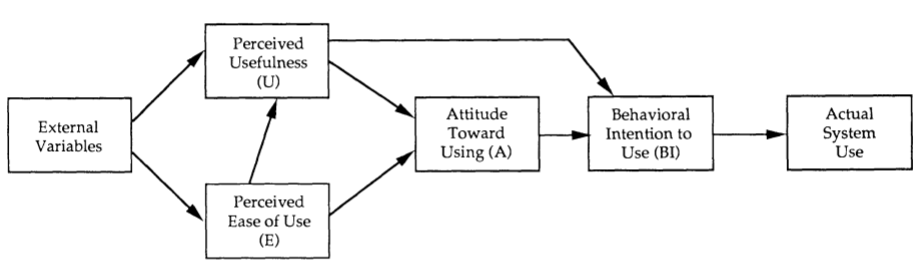
\includegraphics[width=0.8\textwidth]{figures/TAM.png}
  \caption{\acrlong{TAM} \parencite{Davis.1989b} } \label{fig:tam}
\end{figure}

Based on the findings from the interviews the variables are discussed that would influence the perceived usefulness and the perceived ease of use of the designed system and an acceptance model is proposed. As users only review authors are considered but there are many potential types users such as journals, universities, research institutes etc. 

\subsection{External Variables}

\subsubsection{Institutional Demand}

The interviews reveal that researchers don't esteem peer review as part of their resume as they don't feel this information is considered by institutions. It is proposed that the institutional demand for peer review records of a researcher will have a positive impact on the perceived usefulness of the system. With higher such demand, researchers would be more inclined towards showcasing their peer reviews in a verifiable way. 

\subsubsection{Significance of Peer Reviews}

A common statement during the interviews was the insignificance of peer reviews in assessments, tenure, and overall researcher reputation. This was also apparent in how researchers include their review work in their resumes, by only sparing little space for this information. The disparity of this perception in the scientific community with the peer review's importance in scientific knowledge generation has been discussed in previous sections. The disparity has caught the attention of the community \parencite{Verissimo.2013, Tennant.2020} and the need for more recognition to peer review is being voiced. Researchers expect their institutions to require and recognize peer review contributions \parencite{Publons.2018} and state they would spend more time on reviews if it was recognized \parencite{Warne.2016}.

The variable is defined broadly as significance of reviews, as this includes both the value researchers give to reviews, the degree of recognition from institutions, and the attitude of the scientific community towards review work of a researcher. As institutional demand is part of the significance of reviews, it is proposed in the model that the institutional demand positively affects the significance of reviews. Besides, more significance of peer review works of a researcher would increase the need for such peer review showcasing and verification systems. Therefore, proposed is that the significance of reviews will have a positive effect on the perceived usefulness of the technology. Interestingly, this is a chicken and egg problem, where the under-utilization of review recognition platforms are due to peer review's insignificance, and peer review's under-recognition is a result of unavailability of ways to demonstrate peer review work. Put other way, there exist the potential of a virtuous feedback loop: more visibility to peer review may foster peer review's significance and more significance of the process would create more demand to use showcasing platforms.

\subsubsection{Open Science Commitment}

Open Science Commitment can be defined as the degree of support of a researcher for open science practices. The designed artifact aims to remove trusted third parties from the review verification process and promote open data and transparency. This aspect is also the main differentiating property of the designed system from the existing ones. Taking this into account and based on the observations during the interviews, it is proposed that open science commitment of a researcher will have a positive impact on the perceived usefulness of the system. This factor would also influence the preference of a user between existing showcasing systems and the designed system. 

\subsubsection{Active Use Requirement}

The majority of the interviewees expressed the need for automation of the user actions on the platform. Researchers don't spend much time on their peer reviews once they write and submit it. As Interviewee 1 said, reviewers just do the review, send it, then move on to other tasks. They don't think about that review anymore. Joao Oliviera also highlighted the importance of effortless usage of the system, saying he also was invited to try an application similar to Reserachgate but did not continue using it as he didn't want to get into the trouble. Either the value added by the platform should be evident to put time on platform's tasks or it should be as effortless as possible. Google Scholar, since it is the primary online profile and shows a scientist's publications and citation metrics, is checked regularly by Interviewee 1 but they almost never spend time on their Publons profile. Based on these observations it is proposed that the active use requirement has a negative effect on the perceived ease of use. The most important component of this would be adding the reviews to the user profile. If this step could be automated, the perceived ease of use would highly increase.


\begin{figure}[htpb]
  \centering
  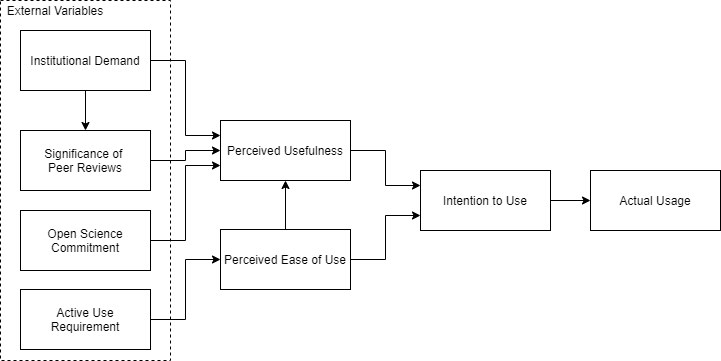
\includegraphics[width=0.8\textwidth]{figures/Proposed TAM.png}
  \caption{Proposed acceptance model for peer review showcasing system } \label{fig:proposed-tam}
\end{figure}

Based on the findings the acceptance model in Figure \ref{fig:proposed-tam} is proposed. The current design requires the reviewer to claim the credentials from their journal and add manually to Veriview. This property falls short in terms of active use requirement and should be improved for a higher perceived ease of use. The rest of the variables are external to the system design and depend on individual users or the wider scientific community. 